%%%%%%%%%%%%%%%%%%%%%%%%%%%%%%%%%%%%%%%%%%%%%%%%%%%%%%%%%%%%%%%%%%%%%%%%%%%%%%%%
%
% FILE: font_free_ocr.tex
%
% DESCRIPTION: LaTeX source file of ICDAR 2007 paper submission
%
% CVS:
% $Id: font_free_ocr.tex,v 1.2 2007-01-12 16:23:21 scottl Exp $
%
%%%%%%%%%%%%%%%%%%%%%%%%%%%%%%%%%%%%%%%%%%%%%%%%%%%%%%%%%%%%%%%%%%%%%%%%%%%%%%%%

% INITIALIZATION %
%%%%%%%%%%%%%%%%%%
\documentclass[times, 10pt,twocolumn]{article} 
\usepackage{latex8}
\usepackage{times}
\usepackage{graphicx}
\pagestyle{empty} %remove page numbers

% DOCUMENT START %
%%%%%%%%%%%%%%%%%%
\begin{document}

% TITLE %
%%%%%%%%%
\title{Font-Free Character Identification for Optical Character Recognition}

% AUTHOUR INFO %
%%%%%%%%%%%%%%%%
\author{First Author\\
Addr 1\\
Addr 2\\
Addr 3\\
\and
Second Author\\
}

%@@the following is not to be included during the review process
%\author{Scott Leishman\\
%Department of Computer Science\\
%University of Toronto\\ 
%scottl@cs.toronto.edu\\
%\and
%Sam Roweis\\
%Department of Computer Science\\
%University of Toronto\\
%roweis@cs.toronto.edu\\
%}

\maketitle
\thispagestyle{empty}


% ABSTRACT %
%%%%%%%%%%%%
\begin{abstract}
@@To be written
\end{abstract}



% INTRODUCTION %
%%%%%%%%%%%%%%%%
\Section{Introduction}

There are several sources of information that play into the optical character
recognition (OCR) pipeline.  At the lowest level, raw pixels and ink patterns
can be used to identify regions corresponding to individual lines, words and
depending on the amount of noise and typeface used, the atomic symbols or
glyphs of a document written in a particular language.  At a higher level, 
structural information like shape, contour, and line offset can be exploited 
to separate and differentiate individual glyphs.  Finally at the highest level 
linguistic or contextual information can be used to refine or improve 
recognized choices.

In carrying out glyph recognition, traditional approaches have typically
been reliant on font information for differentiating glyph shapes; either
by directly comparing component ink blobs to known templates in a particular
size and style, or as input training data for a supervised classifier
or neural network.  Such a reliance often results in degraded performance when 
presented with a document in an unseen font face.

In this paper we take an approach to character recognition that makes no use of
character shape or font, instead relying entirely on contextual and language
cues to recognize characters.

Previous attempts to tackle character recognition in a font independent manner
include work by Nagy\cite{nagy1987} and Huang\cite{huang2006}, that started with
an unsupervised clustering of similar shaped components, then treated this
sequence of cluster identification numbers as a cryptogram to be decoded to the
plain text sequence of output characters.  Ho \cite{ho2000} has taken an
approach that also starts by clustering similar shaped components, then
attempts to infer cluster to character mappings using several simple
statistical modules.  Each module scores assignments based on the ratio of the
number of partially assigned words that match those in a dictionary.

In our approach, we also start by clustering components in an unsupervised
manner.  However, to convert a sequence of clusters to characters, we make use 
of positional statistics as taken from a large textual corpus in the same 
language as the document to be recognized.  In documents written in the 
English language, we know that certain characters like {\em e, a, n} appear 
much more frequently than characters like {\em j, q, X}.  We also know of 
certain character positional regularities, like upper-case letters occurring in 
the first position of a word, or words ending in typical suffices like {\em s, 
ed}.  Furthermore, we know that short stop-words like {\em the, and, of} tend 
to dominate word frequencies in English language texts following a Zipfian 
distribution.



% CLUSTERING APPROACH %
%%%%%%%%%%%%%%%%%%%%%%%
\Section{Clustering Procedure}

In our approach, we must first group together similar blobs of ink on a
page, ideally corresponding to individual characters before we attempt to
recognize them using contextual information.  While we assume in our
experiments that the input consists of bitonal page images in the English 
language, previous work has shown that it is possible to automatically infer 
the script and language of a document based on character shape information
alone\cite{sibun1994},\cite{hochberg1997}.  @@It should also be noted that we
assume typical pre-processing procedures like deskewing, noise removal, and
region identification are performed.@@

An initial set of ink blobs are found by determining the connected components
on each page to be recognized.  For each component, we also store the nearest
neighboring component in each of the four principal directions (top, bottom, 
left, and right).  To determine line boundaries, neighboring components are 
followed in reading order, and their bottom neighbors are checked to see if 
they belong to the same line (share a common left or right component in
following neighboring left or right components).

Since some characters like {\em i, j, \'{e}, :, !} are made up of more than one
connected component, attempts are made to merge their constituent parts.  This 
is accomplished by looking for separate components that belong to the same line,
are separated by a relatively small vertical distance (set manually), and one
of the components completely overlaps the other horizontally.  @@figure showing
this?@@

Each connected component image is initially assigned to its own cluster, then
clusters are merged in a hierarchical fashion.  First a simple Euclidean
distance measurement is taken between cluster centroid images, and those whose
distance falls below a conservatively set threshold are merged together.  For
near noiseless documents, this has the effect of greatly reducing the number of
remaining clusters in a fairly efficient manner, though it has only a slight
impact on noisy documents whose character shapes often vary slightly.

In calculating the Euclidean distance between two images, each pixel difference
is weighted equally regardless of where it occurs.  Thus noisy images
of the same character @@figure??@@ could potentially end up having a larger
distance than two images of differing characters.  To attempt to combat this, 
the clusters are refined using the Hausdorff distance\cite{rucklidge1996}.  

The Hausdorff distance between two binary images $A$ and $B$ is typically 
defined as
\begin{eqnarray}
H(A,B) & = & \max(h(A,B), h(B,A))
\end{eqnarray}
where
\begin{eqnarray}
h(A,B) & = & \max_{a \in A} \min_{b \in B} || a - b ||
\end{eqnarray}
and $|| \cdot ||$ will be the $L_2$ (Euclidean) norm.

$h(A,B)$ can be interpreted as the directed Hausdorff distance from image $A$ to
image $B$, and means that for each foreground pixel in $A$ there is a foreground
pixel in $B$ that is no farther than $h(A,B)$ away, when the two images are 
laid over top one another.

To speed up processing, the Hausdorff distance is only calculated at the most 
correlated position between each cluster centroid image.  This is found by 
convolving the comparison image, with the glued-together image of the other 
clusters.  A Euclidean distance transform is than calculated on the large
glued-together image, then the values at the 'on' pixels of the comparison
image are read off, with the maximum defining the direction Hausdorff distance
from the comparison image to the others.  The Euclidean distance transform is
then calculated on the comparison image, and a large tiled version is
constructed so that 'on' pixels in the other images can be read off to
determine the distance in the other direction.  The maximum of these two
values is then taken to be the overall Hausdorff distance between a comparison
image and the others.  Those that fall within a threshold of @@$\sqrt 2$@@
are then clustered together.

Depending on the font face, amount of kerning employed, and quality of the 
scanned images, some characters may be broken into two or more pieces, or they
may end up touching one another resulting in a single component containing
multiple characters.

To handle characters that have been broken apart, we attempt to merge them by
examining the clusters that they belong to.  If components belonging to a
particular cluster tend to always lie adjacent to components in a second
cluster, and the typical distance between these components is small, then they
are considered for merging.  Components that fall within distance thresholds,
and, of which at least @@85%@@ belong to a cluster that has the same
neighboring cluster are merged.

To handle horizontally touching characters, a recursive procedure is employed.  
For each cluster centroid, we scan across the image, attempting to find a left
and right matching cluster that falls within a particular Euclidean distance.
If we find a match for the left half, we recursively try to split the right
half into at most @@2@@ pieces looking for other cluster matches.

@@We do not make attempts to normalize characters since the Hausdorff distance
combined with centroid pixel averaging can typically be used to catch small
deviations in point size.  Those that vary drastically will end up being left
in separate clusters, however they should still be identified correctly using
contextual procedures.@@

This Hausdorff match, merge, and split procedure is repeated over those 
clusters that have had at least one of their components added or removed during
a particular iteration until no further changes are made.

\begin{figure}[ht]
  \centering
  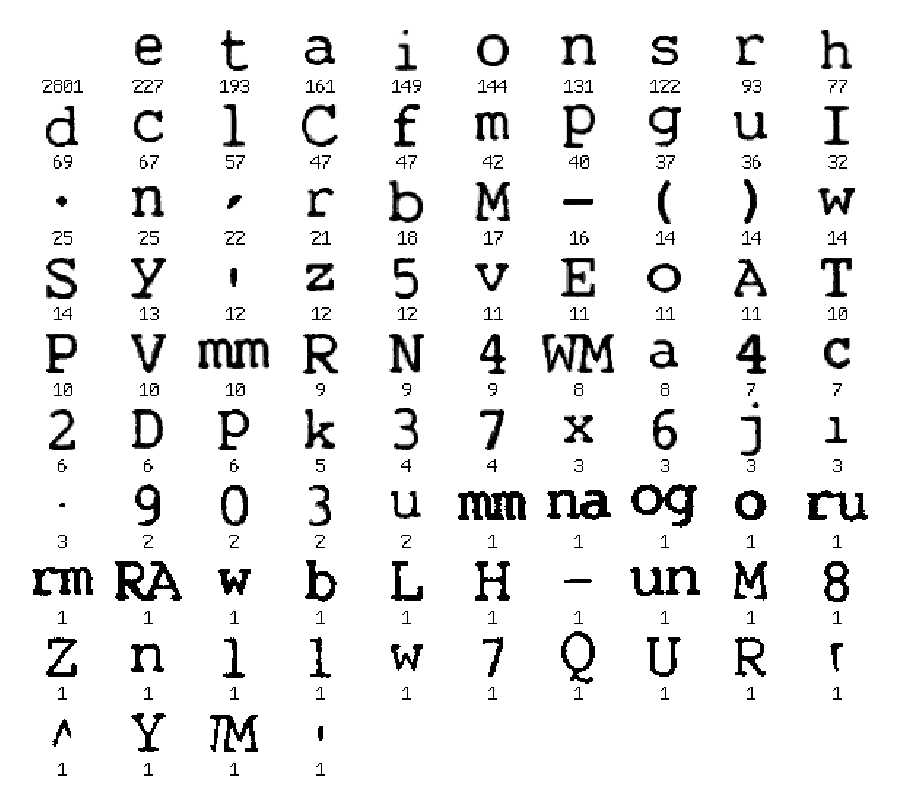
\includegraphics[scale=.5]{figures/cluster_averages}
  \caption{Typical cluster centroids for a single document}
  \label{clavg_fig}
\end{figure}

The last step in the clustering procedure involves the estimation and modeling
of space characters.  We estimate the width of a space character in a simple
fashion by counting the frequency of component neighbor distances.  The first
mode will typically represent inter-character spacing, with a second mode 
representing inter-word spaces.  Space width is calculated based on the point at
which the second mode occurs, but underestimated slightly to ensure no actual
between word spaces are missed.  A new cluster is created to house space
components, and neighbors are updated appropriately.

Figure \ref{clavg_fig} shows the resulting cluster centroids after this
processing has taken place for a typical document in the Reuters-21578 news
corpus\cite{lewis2004}.


% CONTEXTUAL RECOGNITION APPROACH %
%%%%%%%%%%%%%%%%%%%%%%%%%%%%%%%%%%%
\Section{Contextual Recognition}

Once a suitable clustering has been carried out using the techniques described
in the previous section, character labels are inferred using contextual
information.

First a large text corpus is used to estimate word and character frequency, as
well as character positional frequency.  We take counts of the number of times
each character appears in each position of words of length @@10@@ or less.
As a result of this, each character will then define a point in a @@55@@
dimensional ``positional'' feature space.  We normalize each positional count by
dividing by the @@total number of characters seen in the corpus@@.

We repeat this process by gathering positional cluster frequency stats using
the space clusters estimated to demarcate word boundaries.  Again calculating
counts for each cluster in each position of cluster sequences of length @@10@@
or less, each cluster becomes a point in the feature space.

Determining which character each cluster belongs to is then a matter of
finding the closest such point in the feature space.  The distance from each
cluster to each character is calculated, and those that have the shortest
distance are taken to be the most likely candidate mappings.

for frequently occurring characters like lowercase vowels and common consonants
like 't', and 'f', the first candidate is typically the correct choice.
However infrequent characters like punctuation, digits, and upper-case
characters are much rarer (or may not appear at all), so their closest matches
are less likely to be the correct mapping.

@@Haven't tried this yet!!
An approach like that in Ho\cite{ho2000} is then used to improve results.
Considering cluster in order by their frequence, and starting with the closest 
character (in terms of positional feature distance), final character 
assignments are made to clusters using the ratio of occurrences of cluster 
words in which that cluster appears, to partial assignments (including the 
candidate character label to that cluster) that match valid words from the text 
corpus.  If this ratio exceeds a value of @@75\%@@ then the assignment is taken
to be final.@@


% EXPERIMENTS %
%%%%%%%%%%%%%%%
\Section{Experiments}

To examine the validity of our proposed approach, we ran a series of tests 
against the Department of Energy (DOE) Sample 3 dataset from ISRI OCR 
dataset\cite{nartker2005}.  This set consists of 785 pages of ground-truth
labelled document images covering technical reports scanned in varying degrees
of quality, and written in the English language.  This dataset typically does 
not contain entire documents, instead only a small random subset (often on the
order of a few pages) is included.

We grouped all the pages belonging to the same document together and proceeded
to cluster the ink in the textual regions identified by each pages zoning file.

To make use of contextual information, we made use of the first piece of the
Reuters-21578 news corpus\cite{lewis2004}.  After extracting the tags and
trailing ``Reuters'' line from each article we were left with 17601 unique
words including many proper nouns, digit strings, and other non-dictionary
words.  By extracting positional counts for each of 92 different symbols in the
744522 characters of text we were able to create feature vectors for each
symbol that we could then map clusters to.

After determining a mapping from each cluster to a symbol in the document, the
results were compared with the ground-truth text to determine the accuracy.
Figure \ref{characc_fig} shows the character accuracy as compared with document
size by just taking the closest map in feature space.  While spaces, lowercase
vowels and other frequently occuring characters were often found with
relatively high accuracy, most of the symbols in the document were incorrectly
labelled.  @@Only plotted for 191 documents thus far@@

\begin{figure}[ht]
  \centering
  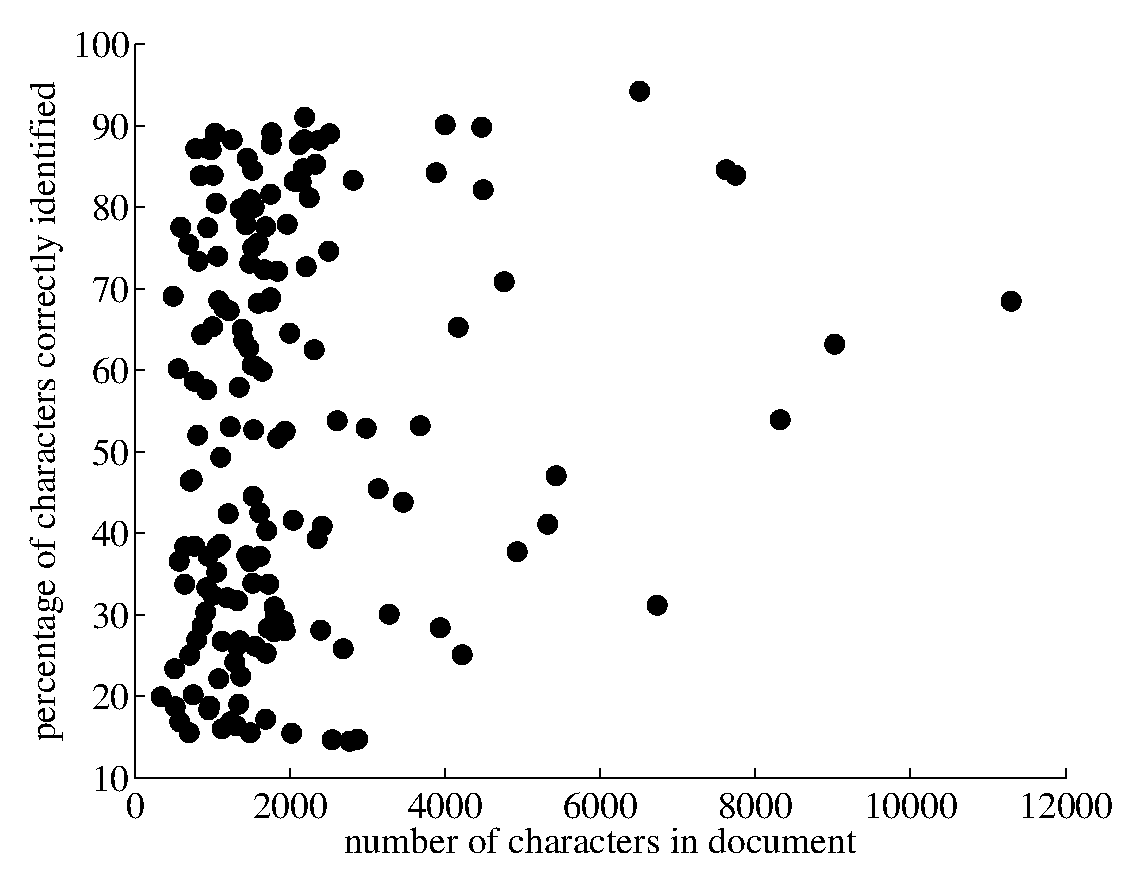
\includegraphics[scale=.4]{figures/character_accuracy}
  \caption{Scatter plot showing character accuracy versus document size}
  \label{characc_fig}
\end{figure}

As a comparison, Figure \ref{gtcharacc_fig} shows the character accuracy by
clustering together the ground-truth text symbols in each document.  The
documents varied in length from 10 characters to 37,000 characters (averaging
around 3,000 characters per document).  
mean document accuracy of just 10\%.

\begin{figure}[ht]
  \centering
  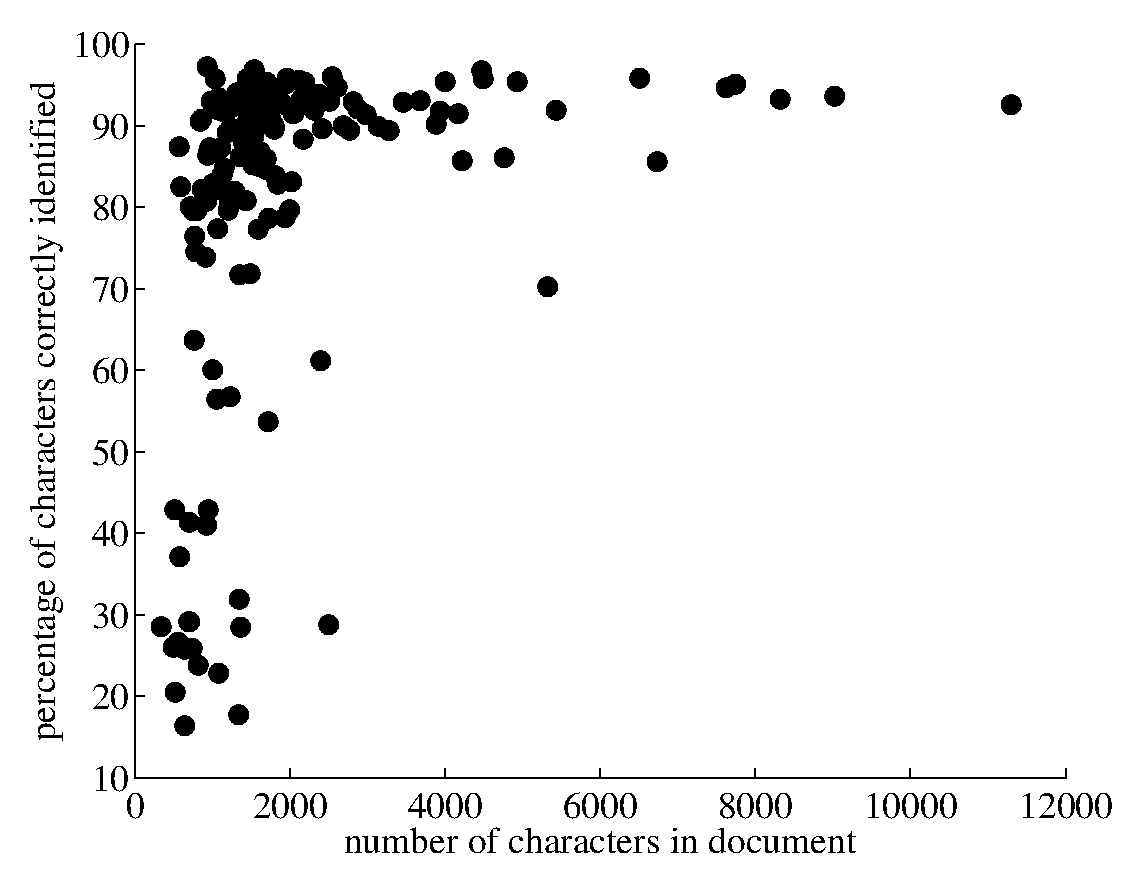
\includegraphics[scale=.4]{figures/gt_character_accuracy}
  \caption{Scatter plot showing ground-truth cluster character accuracy versus 
           document size}
  \label{gtcharacc_fig}
\end{figure}


% CONCLUSIONS %
%%%%%%%%%%%%%%%
\Section{Conclusions}
@@To be written.@@


% REFERENCES %
%%%%%%%%%%%%%%
\bibliographystyle{latex8}
\bibliography{font_free_ocr}

\end{document}
